\chapter{Descripción de la realización}

\section{Método de desarrollo}

En el EDT del proyecto (Figura~\ref{fig:edt}) podemos ver cómo se realizará el proyecto, y cómo se
hará la subdivisión de las tareas.

\begin{figure}
	\centering
	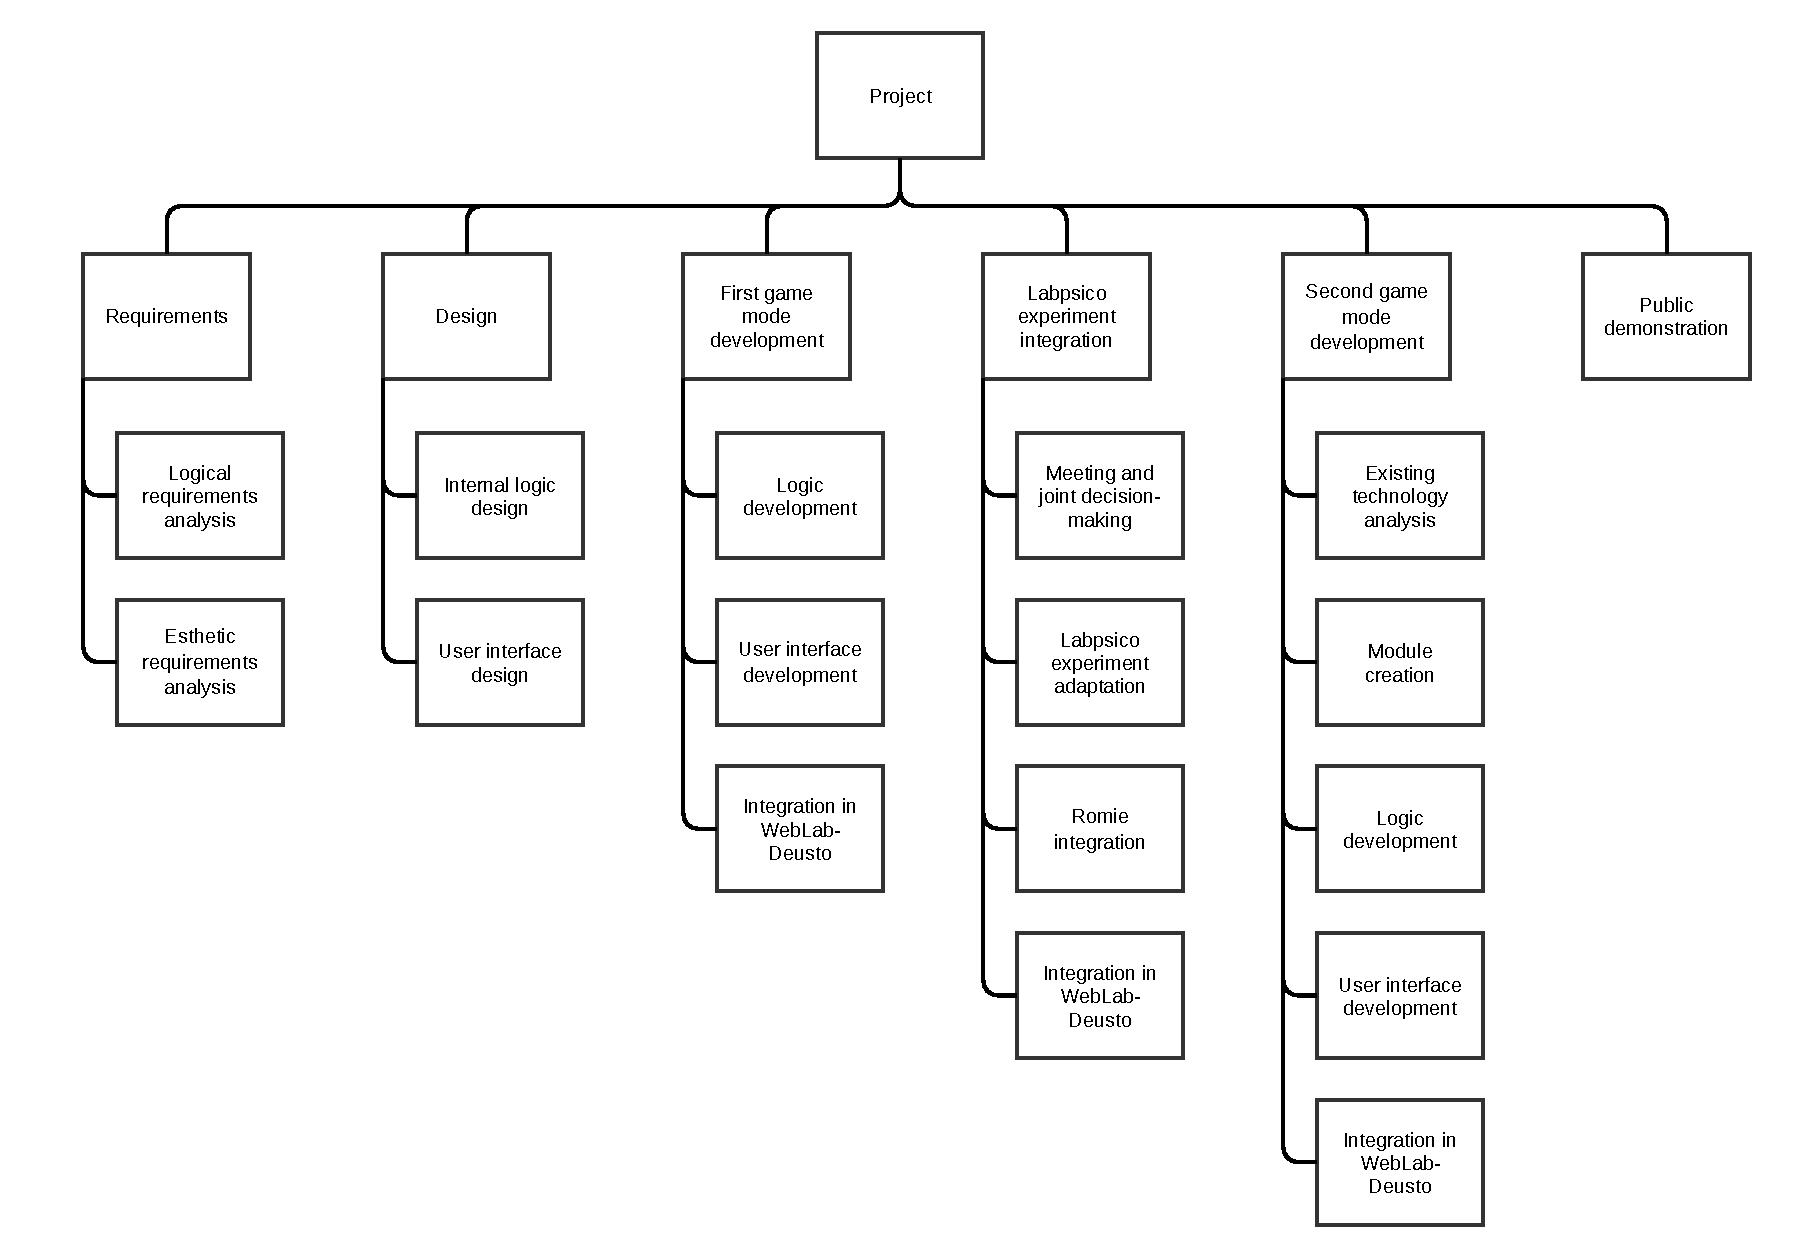
\includegraphics[height=\textwidth, angle=-90]{fig/edt}
	\caption{EDT del proyecto.}\label{fig:edt}
\end{figure}

Como se puede ver en el EDT, las fases del proyecto son las siguientes:

\begin{itemize}
\item \textbf{Requisitos}: Análisis de requisitos del proyecto, en el que se determinarán cuales
serán los requisitos funcionales y estéticos del proyecto.

\item \textbf{Diseño}: Exhaustivo diseño del proyecto, tanto funcional como estético, para definir
cómo será el producto final.

\item \textbf{Creación de la primera modalidad de juego}: Se creará el primer producto intermedio,
y se integrará con la plataforma Weblab-Deusto.

\item \textbf{Integración con el experimento de Labpsico}: Se integrará con la primera modalidad de
juego un experimento psicológico proporcionado por el laboratorio de psicología de Deusto, Labpsico.

\item \textbf{Creación de la segunda modalidad de juego}: Se creará la segunda modalidad de juego,
basada en la programación visual, para ayuda al aprendizaje de lógica computacional.

\item \textbf{Demostración pública}: Se demostrará públicamente con alumnos de primaria y secundaria
para comprobar la viabilidad y fiabilidad del proyecto.
\end{itemize}

\subsection{Productos intermedios}

Estos serán los productos intermedios de los que se compondrá el proyecto:

\begin{itemize}
\item \textbf{Primera modalidad de juego}: Un juego tipo trivial en el que el usuario moverá el
robot por un laberinto y responderá preguntas en lugares concretos.

\item \textbf{Modalidad con experimento de Labpsico}: El mismo juego de la primera modalidad de
juego,  precedido por una completa experiencia psicológica de lucha contra la pseudociencia.

\item \textbf{Segunda modalidad de juego}: Se creará una modalidad de juego que permitirá a los
usuarios programar acciones del robot y hacerlo moverse por el laberinto, con simples retos.
\end{itemize}

\section{Tareas principales}

\subsection{Requisitos}

\begin{itemize}
\item \textbf{T1 - Análisis de requisitos lógicos}: Se debe hacer un análisis detallado de todos los
requisitos funcionales de la plataforma, para poder hacer un posterior seguimiento y comprobar su
cumplimiento.

\item \textbf{T2 - Análisis de requisitos estéticos}: Se debe hacer un análisis detallado de todos
los requisitos estéticos de la plataforma, para poder hacer un posterior seguimiento y comprobar su
cumplimiento.
\end{itemize}

\subsection{Diseño}

\begin{itemize}
\item \textbf{T3 - Diseño de la lógica interna}: Se debe diseñar la lógica interna del robot y de la
plataforma de control del mismo, para hacerla accesible, simple y estable.

\item \textbf{T4 - Diseño de la interfaz}: Se debe hacer un diseño de la interfaz de la plataforma
pensando en el usuario final, para que el robot sea fácil de controlar.
\end{itemize}

\subsection{Creación de la primera modalidad de juego}

\begin{itemize}
\item \textbf{T5 - Creación de la lógica}: Se creará la lógica interna del juego de trivial pensando
siempre en la modularidad y extensibilidad.

\item \textbf{T6 - Creación de la interfaz}: Se creará una interfaz acorde con los estándares de
usabilidad, así como teniendo en cuenta el crédito a los patrocinadores del proyecto.

\item \textbf{T7 - Integración con Weblab-Deusto}: Se integrará la plataforma de juego con
Weblab-Deusto, haciendo uso de su API y sus laboratorios.
\end{itemize}

\subsection{Integración con el experimento de Labpsico}

\begin{itemize}
\item \textbf{T8 - Reunión y toma de decisiones conjunta}: Se hará una reunión con el laboratorio de
psicología de Deusto, Labpsico, en la que se definirá cómo integraremos su experimento con Romie, el
robot que se usará en este proyecto.

\item \textbf{T9 - Adaptación del experimento de Labpsico}: Se adaptará el experimento de Labpsico
para que tenga sentido en el marco de Romie.

\item \textbf{T10 - Integración con Romie}: Se integrará el experimento con la plataforma existente
de Romie, haciendo uso de la interfaz creada para la primera modalidad de juego.

\item \textbf{T11 - Integración con Weblab-Deusto}: Se integrará el nuevo juego con Weblab-Deusto
haciendo uso de sus sistemas de colas y prioridades.
\end{itemize}

\subsection{Creación de la segunda modalidad de juego}

\begin{itemize}
\item \textbf{T12 - Análisis de tecnologías existentes}: Se hará un análisis detallado de las
tecnologías existentes para la programación gráfica, y se decidirá cual será la usada en esta
modalidad.

\item \textbf{T13 - Creación de los módulos básicos}: Se crearán los módulos básicos para programar
el robot.

\item \textbf{T14 - Desarrollo de lógica}: Se desarrollará la lógica interna de la modalidad de
juego, y se decidirá cómo se puntuará.

\item \textbf{T15 - Desarrollo de la interfaz}: Se desarrollará una interfaz sencilla de usar y que
permita acceder a todas las funciones de esta modalidad de juego.

\item \textbf{T16 - Integración con Weblab-Deusto}: Se integrará esta modalidad de juego con
Weblab-Deusto y se hará uso de su sistema de colas y prioridades para compartir el robot.
\end{itemize}

\subsection{Demostración pública}

\begin{itemize}
\item \textbf{T17 - Demostración pública}: Se hará al menos una demostración pública del robot
durante su desarrollo en la que estudiantes lo probarán y jugarán con el.
\end{itemize}

\section{Hojas de tareas}

\subsection{Tarea 1}

\begin{center}
	\begin{tabular}{!{\VRule[4pt]}p{200pt}!{\VRule[2pt]}p{100pt}!{\VRule[4pt]}}
		\specialrule{4pt}{0pt}{0pt}
		\multicolumn{2}{!{\VRule[4pt]}c!{\VRule[4pt]}}{\Large{\textbf{\MakeUppercase{Hoja de tareas}}}} \\
		\specialrule{2pt}{0pt}{0pt}
		\multicolumn{2}{!{\VRule[4pt]}l!{\VRule[4pt]}}{\textbf{Nombre:} Iban Eguia Moraza} \\
		\multicolumn{2}{!{\VRule[4pt]}l!{\VRule[4pt]}}{\textbf{Fecha:} 29 de marzo de 2015} \\
		\specialrule{2pt}{0pt}{0pt}
		\textbf{Identificación de Tarea :  T1} &  \textbf{Duración :  1 día} \\
		\specialrule{4pt}{0pt}{0pt}
	\end{tabular}
\end{center}

\clearpage

\subsection{Tarea 2}

{
\fontfamily{cmss}
\setlength{\extrarowheight}{4pt}
\begin{center}
	\begin{tabular}{!{\VRule[4pt]}p{200pt}!{\VRule[2pt]}p{100pt}!{\VRule[4pt]}}
		\specialrule{4pt}{0pt}{0pt}
		\multicolumn{2}{!{\VRule[4pt]}c!{\VRule[4pt]}}{\Large{\textbf{\MakeUppercase{Hoja de tareas}}}} \\
		\specialrule{2pt}{0pt}{0pt}
		\multicolumn{2}{!{\VRule[4pt]}l!{\VRule[4pt]}}{\textbf{Nombre:} Iban Eguia Moraza} \\
		\multicolumn{2}{!{\VRule[4pt]}l!{\VRule[4pt]}}{\textbf{Fecha:} 29 de marzo de 2015} \\
		\specialrule{2pt}{0pt}{0pt}
		\multirowcell{2}{\textbf{Identificación de Tarea : T2}\\
		\textbf{Descripción:}\\
		Se debe hacer un análisis detallado de todos los requisitos estéticos de la plataforma, para
		poder hacer un posterior seguimiento y comprobar su cumplimiento.}%}%
		                                                      & \makecell{ \\[-1.5ex]\textbf{Duración : 1 día}\vskip0.5ex} \\
		\Xcline{2-2}{2pt}
		%
		                                                      & \makecell{ \\[-0.5ex]\textbf{Esfuerzo: 2 horas}\vskip0.5ex} \\
		\Xcline{2-2}{2pt}
		%
		                                                      & \multirowcell{2}{\textbf{Tareas previas:}} \\
		\Xcline{1-1}{2pt}
		%\multirowcell{2}{
		\textbf{Criterios de terminación:} & \\
		Se creará un informe de requisitos estéticos de la aplicación. El comité de dirección será
		el encargado de validar y aceptar la tarea.
		                                                      & \\[-3ex]
		\Xcline{2-2}{2pt}
		                                                      & \multirowcell{2}{\textbf{Recursos:}\\
		                                                      	Jefe de proyecto} \\
		\Xcline{1-1}{2pt}
		\textbf{Competencias, conocimientos y notas:} & \\
		%%
		{Se debe conocer la materia en la que se trabaja para conocer los requerimientos que se
		necesitan para su completación.} & \\
		\specialrule{4pt}{0pt}{0pt}
	\end{tabular}
\end{center}
}

\clearpage

\subsection{Tarea 3}

{
\fontfamily{cmss}
\setlength{\extrarowheight}{4pt}
\begin{center}
	\begin{tabular}{!{\VRule[4pt]}p{200pt}!{\VRule[2pt]}p{100pt}!{\VRule[4pt]}}
		\specialrule{4pt}{0pt}{0pt}
		\multicolumn{2}{!{\VRule[4pt]}c!{\VRule[4pt]}}{\Large{\textbf{\MakeUppercase{Hoja de tareas}}}} \\
		\specialrule{2pt}{0pt}{0pt}
		\multicolumn{2}{!{\VRule[4pt]}l!{\VRule[4pt]}}{\textbf{Nombre:} Iban Eguia Moraza} \\
		\multicolumn{2}{!{\VRule[4pt]}l!{\VRule[4pt]}}{\textbf{Fecha:} 29 de marzo de 2015} \\
		\specialrule{2pt}{0pt}{0pt}
		\multirowcell{2}{\textbf{Identificación de Tarea : T3}\\
		\textbf{Descripción:}\\
		Se debe diseñar la lógica interna del robot y de la plataforma de control del mismo, para
		hacerla accesible, simple y estable.}
		                                                      & \makecell{ \\[-1.5ex]\textbf{Duración : 8 días}\vskip0.5ex} \\
		\Xcline{2-2}{2pt}

		                                                      & \makecell{ \\[-0.5ex]\textbf{Esfuerzo: 32 horas}\vskip0.5ex} \\
		\Xcline{2-2}{2pt}

		                                                      & \multirowcell{2}{\textbf{Tareas previas:} \\
		                                                      	T1} \\
		\Xcline{1-1}{2pt}

		\textbf{Criterios de terminación:} & \\
		El robot será controlable mediante comandos. El comité de dirección será el encargado de
		validar y aceptar la tarea.
		                                                      & \\[-3ex]
		\Xcline{2-2}{2pt}
		                                                      & \multirowcell{2}{\textbf{Recursos:}\\
		                                                      	Programador} \\
		\Xcline{1-1}{2pt}
		\textbf{Competencias, conocimientos y notas:} & \\

		{El programador deberá conocer el funcionamiento del robot, así como la estuctura del
		laberinto. Además, deberá ser capaz de programarlo y de solucionar problemas que pudieran
		ocurrir.} & \\
		\specialrule{4pt}{0pt}{0pt}
	\end{tabular}
\end{center}
}

\clearpage

\subsection{Tarea 4}

{
\fontfamily{cmss}
\setlength{\extrarowheight}{4pt}
\begin{center}
	\begin{tabular}{!{\VRule[4pt]}p{200pt}!{\VRule[2pt]}p{100pt}!{\VRule[4pt]}}
		\specialrule{4pt}{0pt}{0pt}
		\multicolumn{2}{!{\VRule[4pt]}c!{\VRule[4pt]}}{\Large{\textbf{\MakeUppercase{Hoja de tareas}}}} \\
		\specialrule{2pt}{0pt}{0pt}
		\multicolumn{2}{!{\VRule[4pt]}l!{\VRule[4pt]}}{\textbf{Nombre:} Iban Eguia Moraza} \\
		\multicolumn{2}{!{\VRule[4pt]}l!{\VRule[4pt]}}{\textbf{Fecha:} 29 de marzo de 2015} \\
		\specialrule{2pt}{0pt}{0pt}
		\multirowcell{2}{\textbf{Identificación de Tarea : T4}\\
		\textbf{Descripción:}\\
		Se debe diseñar la lógica interna del robot y de la plataforma de control del mismo, para
		hacerla accesible, simple y estable.}
		                                                      & \makecell{ \\[-1.5ex]\textbf{Duración : 4 días}\vskip0.5ex} \\
		\Xcline{2-2}{2pt}

		                                                      & \makecell{ \\[-0.5ex]\textbf{Esfuerzo: 16 horas}\vskip0.5ex} \\
		\Xcline{2-2}{2pt}

		                                                      & \multirowcell{2}{\textbf{Tareas previas:} \\
		                                                      	T2} \\
		\Xcline{1-1}{2pt}

		\textbf{Criterios de terminación:} & \\
		Habrá una interfaz funcional capaz de comunicarse con el robot. El comité de dirección será
		el encargado de validar y aceptar la tarea.
		                                                      & \\[-3ex]
		\Xcline{2-2}{2pt}
		                                                      & \multirowcell{2}{\textbf{Recursos:}\\
		                                                      	Diseñador} \\
		\Xcline{1-1}{2pt}
		\textbf{Competencias, conocimientos y notas:} & \\

		{El diseñador deberá conocer cómo crear un diseño útil, simple y fácil de usar, para
		permitir a los usuarios acceder a la API del robot fácilmente.} & \\
		\specialrule{4pt}{0pt}{0pt}
	\end{tabular}
\end{center}
}

\clearpage

\subsection{Tarea 5}

{
\fontfamily{cmss}
\setlength{\extrarowheight}{4pt}
\begin{center}
	\begin{tabular}{!{\VRule[4pt]}p{200pt}!{\VRule[2pt]}p{100pt}!{\VRule[4pt]}}
		\specialrule{4pt}{0pt}{0pt}
		\multicolumn{2}{!{\VRule[4pt]}c!{\VRule[4pt]}}{\Large{\textbf{\MakeUppercase{Hoja de tareas}}}} \\
		\specialrule{2pt}{0pt}{0pt}
		\multicolumn{2}{!{\VRule[4pt]}l!{\VRule[4pt]}}{\textbf{Nombre:} Iban Eguia Moraza} \\
		\multicolumn{2}{!{\VRule[4pt]}l!{\VRule[4pt]}}{\textbf{Fecha:} 29 de marzo de 2015} \\
		\specialrule{2pt}{0pt}{0pt}
		\multirowcell{2}{\textbf{Identificación de Tarea : T5}\\
		\textbf{Descripción:}\\
		Se creará la lógica interna del juego de trivial pensando siempre en la modularidad y
		extensibilidad.}
		                                                      & \makecell{ \\[-1.5ex]\textbf{Duración : 14 días}\vskip0.5ex} \\
		\Xcline{2-2}{2pt}

		                                                      & \makecell{ \\[-0.5ex]\textbf{Esfuerzo: 56 horas}\vskip0.5ex} \\
		\Xcline{2-2}{2pt}

		                                                      & \multirowcell{2}{\textbf{Tareas previas:} \\
		                                                      	T3} \\
		\Xcline{1-1}{2pt}

		\textbf{Criterios de terminación:} & \\
		Habrá un juego tipo trivial en el que se podrá jugar y responder preguntas para alcanzar
		altas puntuaciones. El comité de dirección será el encargado de validar y aceptar la tarea.
		                                                      & \\[-3ex]
		\Xcline{2-2}{2pt}
		                                                      & \multirowcell{2}{\textbf{Recursos:}\\
		                                                      	Programador} \\
		\Xcline{1-1}{2pt}
		\textbf{Competencias, conocimientos y notas:} & \\

		{El programador ha de conocer los conceptos relacionados con la gamificación y aplicarlos
		para crear un juego divertido e interesante.} & \\
		\specialrule{4pt}{0pt}{0pt}
	\end{tabular}
\end{center}
}

\clearpage

\subsection{Tarea 6}

{
\fontfamily{cmss}
\setlength{\extrarowheight}{4pt}
\begin{center}
	\begin{tabular}{!{\VRule[4pt]}p{200pt}!{\VRule[2pt]}p{100pt}!{\VRule[4pt]}}
		\specialrule{4pt}{0pt}{0pt}
		\multicolumn{2}{!{\VRule[4pt]}c!{\VRule[4pt]}}{\Large{\textbf{\MakeUppercase{Hoja de tareas}}}} \\
		\specialrule{2pt}{0pt}{0pt}
		\multicolumn{2}{!{\VRule[4pt]}l!{\VRule[4pt]}}{\textbf{Nombre:} Iban Eguia Moraza} \\
		\multicolumn{2}{!{\VRule[4pt]}l!{\VRule[4pt]}}{\textbf{Fecha:} 29 de marzo de 2015} \\
		\specialrule{2pt}{0pt}{0pt}
		\multirowcell{2}{\textbf{Identificación de Tarea : T6}\\
		\textbf{Descripción:}\\
		Se creará una interfaz acorde con los estándares de usabilidad, así como teniendo en cuenta
		el crédito a los patrocinadores del proyecto.}
		                                                      & \makecell{ \\[-1.5ex]\textbf{Duración : 7 días}\vskip0.5ex} \\
		\Xcline{2-2}{2pt}

		                                                      & \makecell{ \\[-0.5ex]\textbf{Esfuerzo: 28 horas}\vskip0.5ex} \\
		\Xcline{2-2}{2pt}

		                                                      & \multirowcell{2}{\textbf{Tareas previas:} \\
		                                                      	T4} \\
		\Xcline{1-1}{2pt}

		\textbf{Criterios de terminación:} & \\
		Habrá un juego fácil de usar, haciendo uso de la lógica del juego. Permitirá a los usuarios
		acceder a todas las funciones fácilmente. El comité de dirección será el encargado de
		validar y aceptar la tarea.
		                                                      & \\[-3ex]
		\Xcline{2-2}{2pt}
		                                                      & \multirowcell{2}{\textbf{Recursos:}\\
		                                                      	Diseñador} \\
		\Xcline{1-1}{2pt}
		\textbf{Competencias, conocimientos y notas:} & \\

		{El diseñador deberá conocer los conceptos relacionados con el responsive design y deberá
		saber cómo realizar una correcta interfaz de usuario.} & \\
		\specialrule{4pt}{0pt}{0pt}
	\end{tabular}
\end{center}
}

\clearpage

\subsection{Tarea 7}

{
\fontfamily{cmss}
\setlength{\extrarowheight}{4pt}
\begin{center}
	\begin{tabular}{!{\VRule[4pt]}p{200pt}!{\VRule[2pt]}p{100pt}!{\VRule[4pt]}}
		\specialrule{4pt}{0pt}{0pt}
		\multicolumn{2}{!{\VRule[4pt]}c!{\VRule[4pt]}}{\Large{\textbf{\MakeUppercase{Hoja de tareas}}}} \\
		\specialrule{2pt}{0pt}{0pt}
		\multicolumn{2}{!{\VRule[4pt]}l!{\VRule[4pt]}}{\textbf{Nombre:} Iban Eguia Moraza} \\
		\multicolumn{2}{!{\VRule[4pt]}l!{\VRule[4pt]}}{\textbf{Fecha:} 29 de marzo de 2015} \\
		\specialrule{2pt}{0pt}{0pt}
		\multirowcell{2}{\textbf{Identificación de Tarea : T7}\\
		\textbf{Descripción:}\\
		Se integrará la plataforma de juego con Weblab-Deusto, haciendo uso de su API y sus
		laboratorios.}
		                                                      & \makecell{ \\[-1.5ex]\textbf{Duración : 8 días}\vskip0.5ex} \\
		\Xcline{2-2}{2pt}

		                                                      & \makecell{ \\[-0.5ex]\textbf{Esfuerzo: 32 horas}\vskip0.5ex} \\
		\Xcline{2-2}{2pt}

		                                                      & \multirowcell{2}{\textbf{Tareas previas:} \\
		                                                      	T5 \\
		                                                      	T6} \\
		\Xcline{1-1}{2pt}

		\textbf{Criterios de terminación:} & \\
		La primera modalidad de juego podrá ser usada por usuarios de WebLab-Deusto y se podrán
		realizar experimentos en producción. El comité de dirección será el encargado de validar y
		aceptar la tarea.
		                                                      & \\[-3ex]
		\Xcline{2-2}{2pt}
		                                                      & \multirowcell{2}{\textbf{Recursos:}\\
		                                                      	\pbox{100pt}{Experto en WebLab-Deusto}} \\
		\Xcline{1-1}{2pt}
		\textbf{Competencias, conocimientos y notas:} & \\

		{El experto deberá conocer cómo realizar una integración de un experimento en los
		laboratorios remotos de Weblab-Deusto, haciendo uso de sus APIs.} & \\
		\specialrule{4pt}{0pt}{0pt}
	\end{tabular}
\end{center}
}

\clearpage

\subsection{Tarea 8}

{
\fontfamily{cmss}
\setlength{\extrarowheight}{4pt}
\begin{center}
	\begin{tabular}{!{\VRule[4pt]}p{200pt}!{\VRule[2pt]}p{100pt}!{\VRule[4pt]}}
		\specialrule{4pt}{0pt}{0pt}
		\multicolumn{2}{!{\VRule[4pt]}c!{\VRule[4pt]}}{\Large{\textbf{\MakeUppercase{Hoja de tareas}}}} \\
		\specialrule{2pt}{0pt}{0pt}
		\multicolumn{2}{!{\VRule[4pt]}l!{\VRule[4pt]}}{\textbf{Nombre:} Iban Eguia Moraza} \\
		\multicolumn{2}{!{\VRule[4pt]}l!{\VRule[4pt]}}{\textbf{Fecha:} 29 de marzo de 2015} \\
		\specialrule{2pt}{0pt}{0pt}
		\multirowcell{2}{\textbf{Identificación de Tarea : T8}\\
		\textbf{Descripción:}\\
		Se hará una reunión con el laboratorio de psicología de Deusto, Labpsico, en la que se
		definirá cómo integraremos su experimento con Romie.}
		                                                      & \makecell{ \\[-1.5ex]\textbf{Duración : 1 día}\vskip0.5ex} \\
		\Xcline{2-2}{2pt}

		                                                      & \makecell{ \\[-0.5ex]\textbf{Esfuerzo: 2 horas}\vskip0.5ex} \\
		\Xcline{2-2}{2pt}

		                                                      & \multirowcell{2}{\textbf{Tareas previas:} \\
		                                                      	T7} \\
		\Xcline{1-1}{2pt}

		\textbf{Criterios de terminación:} & \\
		Se realizará una reunión, y se tomarán todas las decisiones referentes a la integración del
		experimento de Labpsico. El comité de dirección será el encargado de validar y aceptar la
		tarea.
		                                                      & \\[-3ex]
		\Xcline{2-2}{2pt}
		                                                      & \multirowcell{2}{\textbf{Recursos:}\\
		                                                      	Jefe de proyecto} \\
		\Xcline{1-1}{2pt}
		\textbf{Competencias, conocimientos y notas:} & \\

		{El jefe de proyecto deberá demostrar sus competencias de comunicaación y negociación para
		llegar a un acuerdo de colaboración con el laboratorio de psicología Labpsico.} & \\
		\specialrule{4pt}{0pt}{0pt}
	\end{tabular}
\end{center}
}

\clearpage

\subsection{Tarea 9}

{
\fontfamily{cmss}
\setlength{\extrarowheight}{4pt}
\begin{center}
	\begin{tabular}{!{\VRule[4pt]}p{200pt}!{\VRule[2pt]}p{100pt}!{\VRule[4pt]}}
		\specialrule{4pt}{0pt}{0pt}
		\multicolumn{2}{!{\VRule[4pt]}c!{\VRule[4pt]}}{\Large{\textbf{\MakeUppercase{Hoja de tareas}}}} \\
		\specialrule{2pt}{0pt}{0pt}
		\multicolumn{2}{!{\VRule[4pt]}l!{\VRule[4pt]}}{\textbf{Nombre:} Iban Eguia Moraza} \\
		\multicolumn{2}{!{\VRule[4pt]}l!{\VRule[4pt]}}{\textbf{Fecha:} 29 de marzo de 2015} \\
		\specialrule{2pt}{0pt}{0pt}
		\multirowcell{2}{\textbf{Identificación de Tarea : T9}\\
		\textbf{Descripción:}\\
		Se adaptará el experimento de Labpsico para que tenga sentido en el marco de Romie.}
		                                                      & \makecell{ \\[-1.5ex]\textbf{Duración : 2 días}\vskip0.5ex} \\
		\Xcline{2-2}{2pt}

		                                                      & \makecell{ \\[-0.5ex]\textbf{Esfuerzo: 8 horas}\vskip0.5ex} \\
		\Xcline{2-2}{2pt}

		                                                      & \multirowcell{2}{\textbf{Tareas previas:} \\
		                                                      	T8} \\
		\Xcline{1-1}{2pt}

		\textbf{Criterios de terminación:} & \\
		El experimento de Labpsico estará preparado para integrarse con el juego del robot. El
		comité de dirección será el encargado de validar y aceptar la tarea.
		                                                      & \\[-3ex]
		\Xcline{2-2}{2pt}
		                                                      & \multirowcell{2}{\textbf{Recursos:}\\
		                                                      	Programador} \\
		\Xcline{1-1}{2pt}
		\textbf{Competencias, conocimientos y notas:} & \\

		{Se deberá conocer cómo es el funcionamiento interno del experimento de Labpsico, y
		prepararlo tanto funcionalmente como gráficamente para integrarlo con Romie.} & \\
		\specialrule{4pt}{0pt}{0pt}
	\end{tabular}
\end{center}
}

\clearpage

\subsection{Tarea 10}

{
\fontfamily{cmss}
\setlength{\extrarowheight}{4pt}
\begin{center}
	\begin{tabular}{!{\VRule[4pt]}p{200pt}!{\VRule[2pt]}p{100pt}!{\VRule[4pt]}}
		\specialrule{4pt}{0pt}{0pt}
		\multicolumn{2}{!{\VRule[4pt]}c!{\VRule[4pt]}}{\Large{\textbf{\MakeUppercase{Hoja de tareas}}}} \\
		\specialrule{2pt}{0pt}{0pt}
		\multicolumn{2}{!{\VRule[4pt]}l!{\VRule[4pt]}}{\textbf{Nombre:} Iban Eguia Moraza} \\
		\multicolumn{2}{!{\VRule[4pt]}l!{\VRule[4pt]}}{\textbf{Fecha:} 29 de marzo de 2015} \\
		\specialrule{2pt}{0pt}{0pt}
		\multirowcell{2}{\textbf{Identificación de Tarea : T10}\\
		\textbf{Descripción:}\\
		Se integrará el experimento con la plataforma existente de Romie, haciendo uso de la
		interfaz creada para la primera modalidad de juego.}
		                                                      & \makecell{ \\[-1.5ex]\textbf{Duración : 8 días}\vskip0.5ex} \\
		\Xcline{2-2}{2pt}

		                                                      & \makecell{ \\[-0.5ex]\textbf{Esfuerzo: 32 horas}\vskip0.5ex} \\
		\Xcline{2-2}{2pt}

		                                                      & \multirowcell{2}{\textbf{Tareas previas:} \\
		                                                      	T9} \\
		\Xcline{1-1}{2pt}

		\textbf{Criterios de terminación:} & \\
		Se podrá realizar el experimento psicológico directamente desde la primera modalidad de
		juego, recibiendo un bonus de puntuación para el trivial. El comité de dirección será el
		encargado de validar y aceptar la tarea.
		                                                      & \\[-3ex]
		\Xcline{2-2}{2pt}
		                                                      & \multirowcell{2}{\textbf{Recursos:}\\
		                                                      	Programador - 80\% \\
		                                                      	Diseñador - 20\%} \\
		\Xcline{1-1}{2pt}
		\textbf{Competencias, conocimientos y notas:} & \\

		{El programador y el diseñador deberán conocer técnicamente tanto el experimento como la
		primera modalidad de juego para poder integrarlos en una sola aplicación.} & \\
		\specialrule{4pt}{0pt}{0pt}
	\end{tabular}
\end{center}
}

\clearpage

\subsection{Tarea 11}

{
\fontfamily{cmss}
\setlength{\extrarowheight}{4pt}
\begin{center}
	\begin{tabular}{!{\VRule[4pt]}p{200pt}!{\VRule[2pt]}p{100pt}!{\VRule[4pt]}}
		\specialrule{4pt}{0pt}{0pt}
		\multicolumn{2}{!{\VRule[4pt]}c!{\VRule[4pt]}}{\Large{\textbf{\MakeUppercase{Hoja de tareas}}}} \\
		\specialrule{2pt}{0pt}{0pt}
		\multicolumn{2}{!{\VRule[4pt]}l!{\VRule[4pt]}}{\textbf{Nombre:} Iban Eguia Moraza} \\
		\multicolumn{2}{!{\VRule[4pt]}l!{\VRule[4pt]}}{\textbf{Fecha:} 29 de marzo de 2015} \\
		\specialrule{2pt}{0pt}{0pt}
		\multirowcell{2}{\textbf{Identificación de Tarea : T11}\\
		\textbf{Descripción:}\\
		Se integrará el nuevo juego con Weblab-Deusto haciendo uso de sus sistemas de colas y
		prioridades.}
		                                                      & \makecell{ \\[-1.5ex]\textbf{Duración : 4 días}\vskip0.5ex} \\
		\Xcline{2-2}{2pt}

		                                                      & \makecell{ \\[-0.5ex]\textbf{Esfuerzo: 16 horas}\vskip0.5ex} \\
		\Xcline{2-2}{2pt}

		                                                      & \multirowcell{2}{\textbf{Tareas previas:} \\
		                                                      	T10} \\
		\Xcline{1-1}{2pt}

		\textbf{Criterios de terminación:} & \\
		El juego, incluyendo la modalidad con el experimento psicológico estará disponible en
		producción en Weblab-Deusto haciendo uso de colas y prioridades. El comité de dirección será
		el encargado de validar y aceptar la tarea.
		                                                      & \\[-3ex]
		\Xcline{2-2}{2pt}
		                                                      & \multirowcell{2}{\textbf{Recursos:}\\
		                                                      	\pbox{100pt}{Experto en WebLab-Deusto}} \\
		\Xcline{1-1}{2pt}
		\textbf{Competencias, conocimientos y notas:} & \\

		{El experto en Weblab-Deusto deberá conocer las APIs necesarias para conectar el
		experimento, así como tener un conocimiento básico del funcionamiento del mismo.} & \\
		\specialrule{4pt}{0pt}{0pt}
	\end{tabular}
\end{center}
}

\clearpage

\subsection{Tarea 12}

{
\fontfamily{cmss}
\setlength{\extrarowheight}{4pt}
\begin{center}
	\begin{tabular}{!{\VRule[4pt]}p{200pt}!{\VRule[2pt]}p{100pt}!{\VRule[4pt]}}
		\specialrule{4pt}{0pt}{0pt}
		\multicolumn{2}{!{\VRule[4pt]}c!{\VRule[4pt]}}{\Large{\textbf{\MakeUppercase{Hoja de tareas}}}} \\
		\specialrule{2pt}{0pt}{0pt}
		\multicolumn{2}{!{\VRule[4pt]}l!{\VRule[4pt]}}{\textbf{Nombre:} Iban Eguia Moraza} \\
		\multicolumn{2}{!{\VRule[4pt]}l!{\VRule[4pt]}}{\textbf{Fecha:} 29 de marzo de 2015} \\
		\specialrule{2pt}{0pt}{0pt}
		\multirowcell{2}{\textbf{Identificación de Tarea : T12}\\
		\textbf{Descripción:}\\
		Se hará un análisis detallado de las tecnologías existentes para la programación gráfica, y
		se decidirá cual será la usada en esta modalidad.}
		                                                      & \makecell{ \\[-1.5ex]\textbf{Duración : 2 días}\vskip0.5ex} \\
		\Xcline{2-2}{2pt}

		                                                      & \makecell{ \\[-0.5ex]\textbf{Esfuerzo: 8 horas}\vskip0.5ex} \\
		\Xcline{2-2}{2pt}

		                                                      & \multirowcell{2}{\textbf{Tareas previas:} \\
		                                                      	T11} \\
		\Xcline{1-1}{2pt}

		\textbf{Criterios de terminación:} & \\
		Se realizará un informe indicando cual será la tecnología final elegida para la programación
		visual del robot. El comité de dirección será el encargado de validar y aceptar la tarea.
		                                                      & \\[-3ex]
		\Xcline{2-2}{2pt}
		                                                      & \multirowcell{2}{\textbf{Recursos:}\\
		                                                      	Jefe de proyecto} \\
		\Xcline{1-1}{2pt}
		\textbf{Competencias, conocimientos y notas:} & \\

		{El jefe de proyecto se deberá instruir en las tecnologías existentes para la programación
		visual, para lograr tener un punto de vista de experto.} & \\
		\specialrule{4pt}{0pt}{0pt}
	\end{tabular}
\end{center}
}

\clearpage

\subsection{Tarea 13}

{
\fontfamily{cmss}
\setlength{\extrarowheight}{4pt}
\begin{center}
	\begin{tabular}{!{\VRule[4pt]}p{200pt}!{\VRule[2pt]}p{100pt}!{\VRule[4pt]}}
		\specialrule{4pt}{0pt}{0pt}
		\multicolumn{2}{!{\VRule[4pt]}c!{\VRule[4pt]}}{\Large{\textbf{\MakeUppercase{Hoja de tareas}}}} \\
		\specialrule{2pt}{0pt}{0pt}
		\multicolumn{2}{!{\VRule[4pt]}l!{\VRule[4pt]}}{\textbf{Nombre:} Iban Eguia Moraza} \\
		\multicolumn{2}{!{\VRule[4pt]}l!{\VRule[4pt]}}{\textbf{Fecha:} 29 de marzo de 2015} \\
		\specialrule{2pt}{0pt}{0pt}
		\multirowcell{2}{\textbf{Identificación de Tarea : T13}\\
		\textbf{Descripción:}\\
		Se crearán los módulos básicos para programar el robot.}
		                                                      & \makecell{ \\[-1.5ex]\textbf{Duración : 5 días}\vskip0.5ex} \\
		\Xcline{2-2}{2pt}

		                                                      & \makecell{ \\[-0.5ex]\textbf{Esfuerzo: 20 horas}\vskip0.5ex} \\
		\Xcline{2-2}{2pt}

		                                                      & \multirowcell{2}{\textbf{Tareas previas:} \\
		                                                      	T12} \\
		\Xcline{1-1}{2pt}

		\textbf{Criterios de terminación:} & \\
		Los módulos de control del robot para la plataforma seleccionada estarán disponibles para su
		integración con el mismo. El comité de dirección será el encargado de validar y aceptar la
		tarea.
		                                                      & \\[-3ex]
		\Xcline{2-2}{2pt}
		                                                      & \multirowcell{2}{\textbf{Recursos:}\\
		                                                      	Programador} \\
		\Xcline{1-1}{2pt}
		\textbf{Competencias, conocimientos y notas:} & \\

		{El programador deberá conocer el funcionamiento de los sistemas de programación visual
		seleccionados y deberá conocer cómo realizar módulos para posteriormente programar robots.} & \\
		\specialrule{4pt}{0pt}{0pt}
	\end{tabular}
\end{center}
}

\clearpage

\subsection{Tarea 14}

{
\fontfamily{cmss}
\setlength{\extrarowheight}{4pt}
\begin{center}
	\begin{tabular}{!{\VRule[4pt]}p{200pt}!{\VRule[2pt]}p{100pt}!{\VRule[4pt]}}
		\specialrule{4pt}{0pt}{0pt}
		\multicolumn{2}{!{\VRule[4pt]}c!{\VRule[4pt]}}{\Large{\textbf{\MakeUppercase{Hoja de tareas}}}} \\
		\specialrule{2pt}{0pt}{0pt}
		\multicolumn{2}{!{\VRule[4pt]}l!{\VRule[4pt]}}{\textbf{Nombre:} Iban Eguia Moraza} \\
		\multicolumn{2}{!{\VRule[4pt]}l!{\VRule[4pt]}}{\textbf{Fecha:} 29 de marzo de 2015} \\
		\specialrule{2pt}{0pt}{0pt}
		\multirowcell{2}{\textbf{Identificación de Tarea : T14}\\
		\textbf{Descripción:}\\
		Se desarrollará la lógica interna de la modalidad de juego, y se decidirá cómo se puntuará.}
		                                                      & \makecell{ \\[-1.5ex]\textbf{Duración : 5 días}\vskip0.5ex} \\
		\Xcline{2-2}{2pt}

		                                                      & \makecell{ \\[-0.5ex]\textbf{Esfuerzo: 20 horas}\vskip0.5ex} \\
		\Xcline{2-2}{2pt}

		                                                      & \multirowcell{2}{\textbf{Tareas previas:} \\
		                                                      	T13} \\
		\Xcline{1-1}{2pt}

		\textbf{Criterios de terminación:} & \\
		Se creará una modalidad de juego basada en la programación visual. El comité de dirección
		será el encargado de validar y aceptar la tarea.
		                                                      & \\[-3ex]
		\Xcline{2-2}{2pt}
		                                                      & \multirowcell{2}{\textbf{Recursos:}\\
		                                                      	Programador} \\
		\Xcline{1-1}{2pt}
		\textbf{Competencias, conocimientos y notas:} & \\

		{El programador deberá conocer cómo integrar los módulos de programación visual en una web
		interactiva que permita programar el robot.} & \\
		\specialrule{4pt}{0pt}{0pt}
	\end{tabular}
\end{center}
}

\clearpage

\subsection{Tarea 15}

{
\fontfamily{cmss}
\setlength{\extrarowheight}{4pt}
\begin{center}
	\begin{tabular}{!{\VRule[4pt]}p{200pt}!{\VRule[2pt]}p{100pt}!{\VRule[4pt]}}
		\specialrule{4pt}{0pt}{0pt}
		\multicolumn{2}{!{\VRule[4pt]}c!{\VRule[4pt]}}{\Large{\textbf{\MakeUppercase{Hoja de tareas}}}} \\
		\specialrule{2pt}{0pt}{0pt}
		\multicolumn{2}{!{\VRule[4pt]}l!{\VRule[4pt]}}{\textbf{Nombre:} Iban Eguia Moraza} \\
		\multicolumn{2}{!{\VRule[4pt]}l!{\VRule[4pt]}}{\textbf{Fecha:} 29 de marzo de 2015} \\
		\specialrule{2pt}{0pt}{0pt}
		\multirowcell{2}{\textbf{Identificación de Tarea : T15}\\
		\textbf{Descripción:}\\
		Se desarrollará una interfaz sencilla de usar y que permita acceder a todas las funciones de
		esta modalidad de juego.}
		                                                      & \makecell{ \\[-1.5ex]\textbf{Duración : 4 días}\vskip0.5ex} \\
		\Xcline{2-2}{2pt}

		                                                      & \makecell{ \\[-0.5ex]\textbf{Esfuerzo: 16 horas}\vskip0.5ex} \\
		\Xcline{2-2}{2pt}

		                                                      & \multirowcell{2}{\textbf{Tareas previas:} \\
		                                                      	T12} \\
		\Xcline{1-1}{2pt}

		\textbf{Criterios de terminación:} & \\
		Los usuarios podrán programar el robot visualmente para hacerle cumplir los retos
		necesarios. El comité de dirección será el encargado de validar y aceptar la tarea.
		                                                      & \\[-3ex]
		\Xcline{2-2}{2pt}
		                                                      & \multirowcell{2}{\textbf{Recursos:}\\
		                                                      	Diseñador} \\
		\Xcline{1-1}{2pt}
		\textbf{Competencias, conocimientos y notas:} & \\

		{El diseñador deberá conocer el funcionamiento de las APIs de la programación visual, y
		deberá saber cómo integrarlas en una página web.} & \\
		\specialrule{4pt}{0pt}{0pt}
	\end{tabular}
\end{center}
}

\clearpage

\subsection{Tarea 16}

{
\fontfamily{cmss}
\setlength{\extrarowheight}{4pt}
\begin{center}
	\begin{tabular}{!{\VRule[4pt]}p{200pt}!{\VRule[2pt]}p{100pt}!{\VRule[4pt]}}
		\specialrule{4pt}{0pt}{0pt}
		\multicolumn{2}{!{\VRule[4pt]}c!{\VRule[4pt]}}{\Large{\textbf{\MakeUppercase{Hoja de tareas}}}} \\
		\specialrule{2pt}{0pt}{0pt}
		\multicolumn{2}{!{\VRule[4pt]}l!{\VRule[4pt]}}{\textbf{Nombre:} Iban Eguia Moraza} \\
		\multicolumn{2}{!{\VRule[4pt]}l!{\VRule[4pt]}}{\textbf{Fecha:} 29 de marzo de 2015} \\
		\specialrule{2pt}{0pt}{0pt}
		\multirowcell{2}{\textbf{Identificación de Tarea : T16}\\
		\textbf{Descripción:}\\
		Se integrará esta modalidad de juego con Weblab-Deusto y se hará uso de su sistema de colas
		y prioridades para compartir el robot.}
		                                                      & \makecell{ \\[-1.5ex]\textbf{Duración : 12 días}\vskip0.5ex} \\
		\Xcline{2-2}{2pt}

		                                                      & \makecell{ \\[-0.5ex]\textbf{Esfuerzo: 48 horas}\vskip0.5ex} \\
		\Xcline{2-2}{2pt}

		                                                      & \multirowcell{2}{\textbf{Tareas previas:} \\
		                                                      	T14 \\
		                                                      	T15} \\
		\Xcline{1-1}{2pt}

		\textbf{Criterios de terminación:} & \\
		La segunda modalidad de juego estará integrada con Weblab-Deusto y funcionando en
		producción. El comité de dirección será el encargado de validar y aceptar la tarea.
		                                                      & \\[-3ex]
		\Xcline{2-2}{2pt}
		                                                      & \multirowcell{2}{\textbf{Recursos:}\\
		                                                      	\pbox{100pt}{Experto en WebLab-Deusto}} \\
		\Xcline{1-1}{2pt}
		\textbf{Competencias, conocimientos y notas:} & \\

		{El experto deberá saber cómo funciona la lógica interna de la segunda modalidad de juego y
		conocer cual es la mejor manera de integrarla con Weblab-Deusto.} & \\
		\specialrule{4pt}{0pt}{0pt}
	\end{tabular}
\end{center}
}

\clearpage

\subsection{Tarea 17}

{
\fontfamily{cmss}
\setlength{\extrarowheight}{4pt}
\begin{center}
	\begin{tabular}{!{\VRule[4pt]}p{200pt}!{\VRule[2pt]}p{100pt}!{\VRule[4pt]}}
		\specialrule{4pt}{0pt}{0pt}
		\multicolumn{2}{!{\VRule[4pt]}c!{\VRule[4pt]}}{\Large{\textbf{\MakeUppercase{Hoja de tareas}}}} \\
		\specialrule{2pt}{0pt}{0pt}
		\multicolumn{2}{!{\VRule[4pt]}l!{\VRule[4pt]}}{\textbf{Nombre:} Iban Eguia Moraza} \\
		\multicolumn{2}{!{\VRule[4pt]}l!{\VRule[4pt]}}{\textbf{Fecha:} 29 de marzo de 2015} \\
		\specialrule{2pt}{0pt}{0pt}
		\multirowcell{2}{\textbf{Identificación de Tarea : T17}\\
		\textbf{Descripción:}\\
		Se hará al menos una demostración pública del robot durante su desarrollo en la que
		estudiantes lo probarán y jugarán con el.}
		                                                      & \makecell{ \\[-1.5ex]\textbf{Duración : 3 días}\vskip0.5ex} \\
		\Xcline{2-2}{2pt}

		                                                      & \makecell{ \\[-0.5ex]\textbf{Esfuerzo: 12 horas}\vskip0.5ex} \\
		\Xcline{2-2}{2pt}

		                                                      & \multirowcell{2}{\textbf{Tareas previas:} \\
		                                                      	T7} \\
		\Xcline{1-1}{2pt}

		\textbf{Criterios de terminación:} & \\
		Se hará un informe con las estadísticas de uso y se comprobará el funcionamiento de la
		plataforma en un entorno con estudiantes de primaria y secundaria. El comité de dirección
		será el encargado de validar y aceptar la tarea.
		                                                      & \\[-3ex]
		\Xcline{2-2}{2pt}
		                                                      & \multirowcell{2}{\textbf{Recursos:}\\
		                                                      	Jefe de proyecto} \\
		\Xcline{1-1}{2pt}
		\textbf{Competencias, conocimientos y notas:} & \\

		{El jefe de proyecto deberá demostrar sus competencias comunicativas con los estudiantes y
		los posibles profesores que se interesen por el proyecto.} & \\
		\specialrule{4pt}{0pt}{0pt}
	\end{tabular}
\end{center}
}

\clearpage

